\documentclass[conference]{IEEEtran}
\IEEEoverridecommandlockouts
% Based on the official IEEE Conference Template (conference_101719.tex).
\usepackage{cite}
\usepackage{amsmath,amssymb,amsfonts}
\usepackage{algorithmic}
\usepackage{graphicx}
\usepackage{textcomp}
\usepackage{xcolor}
\usepackage{booktabs}
\usepackage{array}
\usepackage{url}
\usepackage[hidelinks]{hyperref}
\usepackage{balance}
\def\BibTeX{{\rm B\kern-.05em{\sc i\kern-.025em b}\kern-.08em
    T\kern-.1667em\lower.7ex\hbox{E}\kern-.125emX}}
\graphicspath{{figs/}{../figs/}}

\newcommand{\dtp}{DRAM$\rightarrow$PIM}
\newcommand{\ptd}{PIM$\rightarrow$DRAM}
\newcommand{\dpp}{DRAM$\leftrightarrow$PIM}

\begin{document}

\title{Reproducing PIM-MMU: A Simulation Study of \\ DRAM--PIM Data-Transfer Acceleration, \\ with a Ragged-Transfer Extension
\thanks{Group 14 course project. Reproduction of D. Lee, B. Hyun, T. Kim, and
M. Rhu, ``PIM-MMU,'' MICRO 2024~\cite{pimmmu}. All real-hardware experiments are
replaced by simulation.}}

\author{\IEEEauthorblockN{Sunil}
\IEEEauthorblockA{\textit{CSE} \\
\textit{IIT Guwahati}\\
Guwahati, India \\
suniljdh2023@gmail.com}
\and
\IEEEauthorblockN{Subham}
\IEEEauthorblockA{\textit{CSE} \\
\textit{IIT Guwahati}\\
Guwahati, India \\
subhamdagar73@gmail.com}
\and
\IEEEauthorblockN{Shrey Chandra}
\IEEEauthorblockA{\textit{CSE} \\
\textit{IIT Guwahati}\\
Guwahati, India \\
shreychandra@gmail.com}
\and
\IEEEauthorblockN{Jagrati}
\IEEEauthorblockA{\textit{CSE} \\
\textit{IIT Guwahati}\\
Guwahati, India \\
jagrati@gmail.com}}
\maketitle

\begin{abstract}
In a memory-bus PIM system like UPMEM, the DRAM and the PIM cores live in
different physical address spaces, so getting a core its input means copying the
data over by hand first. The PIM-MMU paper~\cite{pimmmu} measures that copy and
finds it dominates end-to-end time, then fixes it with three pieces of hardware:
a Data Copy Engine (DCE) that takes the copy off the CPU, a PIM-aware scheduler
(PIM-MS) that reorders the per-bank copies for parallelism, and a dual-mode
mapping unit (HetMap) that restores the fast DRAM mapping the PIM BIOS normally
disables. This work rebuilds the transfer half of that design in simulation. No
simulator was published with the paper, so we wrote our own model on top of
Ramulator's DDR4 engine: a multi-threaded software copier in the style of
UPMEM's AVX runtime, the DCE, PIM-MS as Algorithm~1 describes it, and both
mappings. As the assignment requires, nothing real-hardware is included --- no
PIM kernels, driver, runtime library, power or area, and no PrIM end-to-end
numbers. Our rebuilt PIM-MMU is up to $4.5\times$ faster than the software
baseline moving data into PIM and up to $6.7\times$ faster moving it out, which
sits inside the paper's range. We also recover its least intuitive result: a
bare copy engine, with none of the scheduling, is actually \emph{slower} than
the software it replaces. Where our numbers part company with the paper --- the
mapping, not the scheduler, carries most of the gain on our setup --- we say so
and explain why. We then push past the paper with a feature it cannot express:
\emph{ragged} transfers that drop the per-DPU padding and add largest-remaining
scheduling and size-aware placement, worth up to $10.8\times$ on lopsided
(sparse-matrix-style) partitions.
\end{abstract}

\begin{IEEEkeywords}
processing-in-memory, UPMEM, data transfer, memory scheduling, memory mapping,
Ramulator.
\end{IEEEkeywords}

\section{Introduction and Problem}
Processing-in-memory puts compute logic right beside the DRAM banks, which is
attractive for workloads that spend most of their time waiting on memory. The
commercial memory-bus parts we care about here, UPMEM-PIM~\cite{upmem} in
particular, are built per bank: one small core sits on each bank. That layout
raises an awkward problem. If the host CPU and a bank's own core could both
reach the same bank at once, the memory controller would have to referee them,
and the DDR timing guarantees would break. UPMEM sidesteps this by giving DRAM
and PIM \emph{separate} physical address spaces, so at any instant a bank is
driven by exactly one of them. The price for that simplicity is paid by the
programmer: before a core can work on anything, its input has to be copied from
the DRAM space into the PIM space, and the results copied back out afterwards.
On the PrIM suite the paper clocks this copy at up to $99.7\%$ of runtime, and
$63.7\%$ on average~\cite{prim} --- in other words, the ``transfer'' is often the
program.

The paper~\cite{pimmmu} traces the slowness to three things. First, the copy
runs on the CPU using AVX-512 loads and stores, which is both power-hungry and a
drain on the cores. Second, the per-bank copies are handed to the OS as ordinary
threads, and the OS schedules them for fairness rather than for memory-level
parallelism (MLP), so the memory channels are used unevenly. Third --- and this
one is easy to miss --- the same BIOS change that carves out a separate PIM
address space also turns off the XOR-hashed, MLP-friendly mapping that ordinary
DRAM traffic depends on, so even plain DRAM accesses get slower. PIM-MMU answers
each in turn: a Data Copy Engine (DCE) moves the copy off the CPU, a PIM-aware
scheduler (PIM-MS) reshuffles the independent per-bank copies to fill the
channels, and HetMap runs two address mappings side by side so DRAM keeps its
fast mapping while PIM keeps the localized one it needs.

What follows is our attempt to rebuild the transfer mechanism in a simulator,
check it against the paper, and then take it somewhere the paper does not go.

\section{How PIM-MMU Works}
We summarize the three pieces here because our model has to reproduce each one.

\textbf{The copy engine.} The DCE is a small accelerator mapped into the
memory-controller's address space. The host sets it up once --- handing over a
list of descriptors (where the source is in DRAM, which PIM core it goes to, how
many bytes) --- and then steps back entirely. The engine does the reads, the
writes, and the $8\times8$ byte transpose that UPMEM requires because a data word
is striped across eight chips. No CPU cycles are spent once it starts.

\textbf{The scheduler.} PIM-MS rests on one observation: the per-bank copies
touch disjoint addresses, so nothing forces them into any particular order. The
software baseline never gets to exploit this, because each OS thread only ever
exposes the requests for its own bank. The DCE, by contrast, holds descriptors
for \emph{every} destination bank simultaneously, so it can interleave them. The
paper's Algorithm~1 walks channels first, then bank groups (to stay ahead of the
$t_{CCD}$ column timing), then banks, taking one access granule from a bank unit
before moving to the next.

\textbf{The mapping.} HetMap is simply two mapping functions living together.
DRAM addresses go through an MLP-centric function --- XOR hashing, channel bits
low --- while PIM addresses use a plain \texttt{ChRaBgBkRoCo} ordering that keeps
each core's data inside its own DIMM. The second mapping looks like it should
throttle PIM, but once PIM-MS is doing the ordering it does not, which is the
point the paper makes and our ablation confirms.

\section{Implementation and Setup}
\subsection{What we built}
Since there was no code to start from, we built the transfer model from scratch
and let Ramulator~\cite{ramulator} (commit \texttt{214f635}) handle the parts a
reproduction should not reinvent: the DDR4 bank-state machine and its timing
(ACT/PRE/RD/WR, $t_{RCD}$, $t_{CCD_{S/L}}$, $t_{FAW}$, refresh), FR-FCFS, and the
open-row policy. The division of labor is clean --- Ramulator decides when a
command can issue, and our code decides which commands exist in the first place.
We changed only two lines in Ramulator: one to actually fire the write-completion
callback (the released code comments it out, so a write never signals back to an
external driver), and one to make FR-FCFS the default scheduler, as the paper's
Table~I specifies.

Our driver program (\texttt{pimsim}, $\sim$600 lines of C++) instantiates two
independent sets of Ramulator DDR4 channels, one for DRAM and one for PIM, each
with its own address-mapping function, and steps them in lockstep at the
DDR4-2400 command clock (1.2\,GHz). It models:

\begin{itemize}
\item \textbf{Bank units and transpose.} Eight DPUs (one per x8 chip, same bank
index) form a bank unit. A 64\,B burst to the unit carries 8\,B for each DPU, so
each source line is $8\times8$ transposed into eight PIM bursts, exactly as in
the paper's Fig.~3. We model the transpose as a fixed preprocessing latency.
\item \textbf{Software baseline (``Base'').} Eight cores, a per-core line-fill
buffer (12 outstanding lines), $\sim$15\,ns one-way core$\leftrightarrow$IMC
latency, and an OS round-robin scheduler with a 1.5\,ms time slice and
context-switch cost. One task per bank unit. The default thread-to-unit order
is randomized to emulate an OS that is unaware of PIM; we also test an
oracle interleaved order.
\item \textbf{DCE (``+D'').} A 16\,KB data buffer and 64\,KB address buffer as
in the paper's Table~I, an address-generation unit, and the transpose unit. It
sits at the memory controller, so its on-chip latency is a few cycles.
\item \textbf{PIM-MS (``+P'').} Algorithm~1 of the paper: channel-parallel,
then bank-group interleaving, then bank, with a configurable access granularity.
\item \textbf{Mappings.} DRAM uses either a locality-centric mapping (paper
Fig.~7a) or an MLP-centric mapping with permutation-based XOR
hashing~\cite{xorhash} (Fig.~7b $=$ HetMap). PIM always uses
\texttt{ChRaBgBkRoCo}.
\end{itemize}

\subsection{Configuration}
Table~\ref{tab:cfg} lists the machine. We model 4 DRAM channels and 4 PIM
channels (2 ranks each, 512 DPUs), close to the paper's 3+3-channel server; the
channel-count difference is the main reason some of our absolute ratios differ
(Section~\ref{sec:threats}).

\begin{table}[t]
\centering
\caption{Simulated configuration (follows the paper's Table~I where applicable).}
\label{tab:cfg}
\small
\begin{tabular}{@{}ll@{}}
\toprule
Host MC & 64-entry read/write queues, FR-FCFS, open-row \\
DRAM & DDR4-2400, 4 channels, 2 ranks/ch, x8 \\
PIM & DDR4-2400, 4 channels, 2 ranks/ch, 512 DPUs, x16 \\
DCE & 1.2\,GHz, 16\,KB data buffer, 64\,KB address buffer \\
PIM-MS & Algorithm~1 \\
HetMap & DRAM: MLP-centric+XOR; PIM: \texttt{ChRaBgBkRoCo} \\
\bottomrule
\end{tabular}
\end{table}

\subsection{Ablation naming}
Following the paper we build up additively: \textbf{Base} (software baseline),
\textbf{+D} (add DCE, descriptor-order DMA, no PIM-MS), \textbf{+D+H} (add
HetMap), \textbf{+D+H+P} (add PIM-MS $=$ full PIM-MMU). We add two points the
paper does not isolate: \textbf{+H} (software baseline but with the MLP-centric
DRAM mapping) and \textbf{+D+P} (DCE with PIM-MS but locality DRAM mapping), to
separate the mapping effect from the scheduler effect.

\subsection{What we left out}
Per the assignment, all real-hardware experiments are omitted. Concretely we do
\emph{not} model or measure: the PIM kernel execution itself (the paper measures
it on real UPMEM hardware); the PIM-MMU device driver and user-level runtime
library; CPU power and chip area (McPAT/CACTI); and the end-to-end PrIM
benchmark times. We evaluate only the \dpp{} (and DRAM$\leftrightarrow$DRAM) data
transfer in simulation. Where the paper blends simulation with wall-clock PIM
kernel time, we report transfer throughput alone.

\section{Baseline Results vs.\ the Paper}
\subsection{Throughput vs.\ transfer size}
Figure~\ref{fig:e1} shows throughput normalized to Base for both directions and
five transfer sizes. The headline trends match the paper's Fig.~15(a):

\begin{itemize}
\item \textbf{Full PIM-MMU wins by a wide margin.} \dtp{} improves by up to
$4.5\times$ (at 8\,MB) and \ptd{} by up to $6.7\times$ over Base, with
geometric-mean gains of $3.1\times$ and $3.9\times$ across sizes. The paper
reports average $3.3\times$/$3.8\times$ and transfer-throughput maxima up to
$6.9\times$; our averages and maxima both sit inside that envelope.
\item \textbf{A plain DCE is slower than Base (+D $<$ Base).} This reproduces
the paper's most counter-intuitive ablation finding: the vanilla DCE, acting
like a conventional DMA engine (Intel I/OAT/DSA), loses to the baseline because
the baseline's out-of-order cores issue wide AVX-512 requests aggressively,
whereas the in-order descriptor-walking DCE does not exploit MLP. In our data
+D delivers $\sim$11\,GB/s vs.\ Base's 16--17\,GB/s.
\item \textbf{HetMap alone does not help, PIM-MS unlocks it.} +D+H tracks +D
(both $\sim$11\,GB/s); only when PIM-MS is added does throughput jump. This too
is the paper's message: +D+H is bottlenecked on PIM read/write throughput, and
PIM-MS is what removes that bottleneck.
\end{itemize}

\begin{figure}[t]
\centering
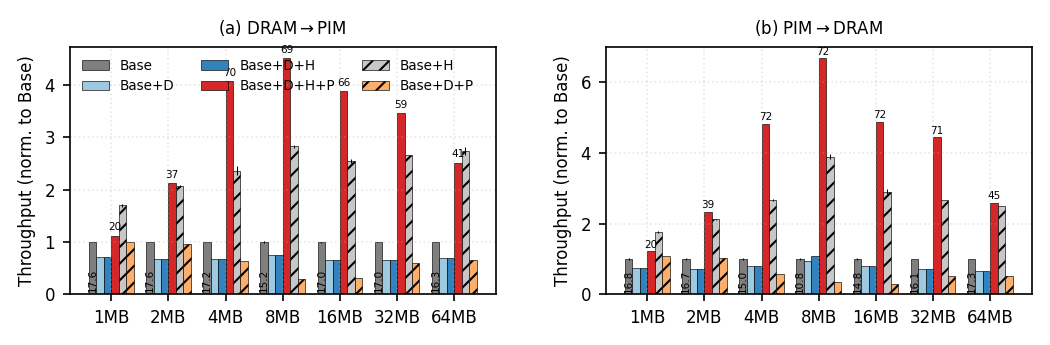
\includegraphics[width=\columnwidth]{e1_throughput_vs_size.png}
\caption{Throughput vs.\ transfer size, normalized to Base (numbers above the
rightmost bars are absolute GB/s for PIM-MMU; small numbers below are Base
GB/s). Compare with the paper's Fig.~15(a).}
\label{fig:e1}
\end{figure}

One number is worth calling out because we did not tune for it. The software
baseline degrades as the transfer grows --- it holds near $16$\,GB/s through
$64$\,MB (the largest size in Fig.~\ref{fig:e1}, which we cap there to keep both
directions on one axis) and bottoms out at $8.3$\,GB/s at $256$\,MB, about
$14\%$ of the $57.6$\,GB/s the channels can deliver. The paper, measuring real
silicon, reports $8.9$\,GB/s and $15.5\%$ utilization for this operation. We were
not aiming at that figure, so having our large-transfer baseline land right next
to it was a good sign that the model captures the right bottleneck. (The
$256$\,MB points are in our data but off the plotted range.)

\subsection{Throughput vs.\ number of PIM modules}
Figure~\ref{fig:e2} scales the PIM capacity from 1 to 4 DIMMs. PIM-MMU's
throughput grows with the channel count and tracks the aggregate PIM-channel
peak, while the software baseline stays flat near $15$\,GB/s regardless of how
many modules are present, because it is limited by CPU-side issue and OS
scheduling rather than by memory bandwidth. Adding ranks without channels does
not raise throughput (ranks add capacity, not bandwidth), matching the paper's
observation for Fig.~14.

\begin{figure}[t]
\centering
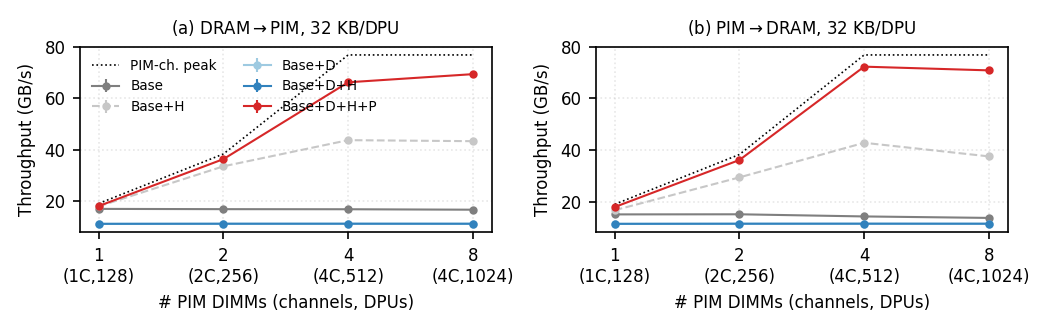
\includegraphics[width=\columnwidth]{e2_modules.png}
\caption{Throughput vs.\ number of PIM DIMMs (channels/DPUs in parentheses),
32\,KB per DPU. PIM-MMU scales with channels; the software baseline is flat.}
\label{fig:e2}
\end{figure}

\subsection{DRAM mapping and HetMap memcpy}
Figure~\ref{fig:e3e4}(a) reproduces the paper's Fig.~8: with the locality-centric
mapping, DRAM bandwidth is a fraction of the MLP-centric mapping across both
sequential and strided access. We observe $\sim$18\% where the paper reports
$\sim$30\%; the gap is explained in Section~\ref{sec:threats}. Fig.~\ref{fig:e3e4}(b)
reproduces Fig.~14: HetMap's MLP-centric DRAM mapping speeds up a
DRAM$\leftrightarrow$DRAM \texttt{memcpy} by $2.3\times$--$4.3\times$ as channels
grow, versus the paper's $4.9\times$ average, and the improvement scales with
channel count as the paper reports.

\begin{figure}[t]
\centering
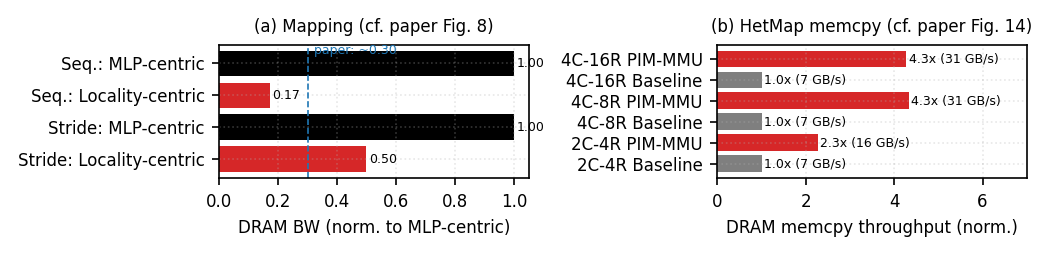
\includegraphics[width=\columnwidth]{e3e4_mapping.png}
\caption{(a) DRAM bandwidth, locality- vs.\ MLP-centric mapping (cf.\ paper
Fig.~8). (b) HetMap \texttt{memcpy} speedup vs.\ channels/ranks (cf.\ Fig.~14).}
\label{fig:e3e4}
\end{figure}

\subsection{Robustness to CPU contention}
Figure~\ref{fig:e5} co-locates the \dtp{} transfer with compute-bound CPU
contenders (paper Fig.~13a). The software baseline's latency rises sharply as
contenders steal the cores its transfer threads need; PIM-MMU stays flat at $0.40\times$ the baseline's zero-contention latency
(a $2.5\times$ speedup that is itself contention-independent), because the copy
runs entirely on the DCE and needs no CPU compute, whereas the baseline degrades
to $1.36\times$ with 24 contenders. This is a
clean qualitative reproduction.

\begin{figure}[t]
\centering
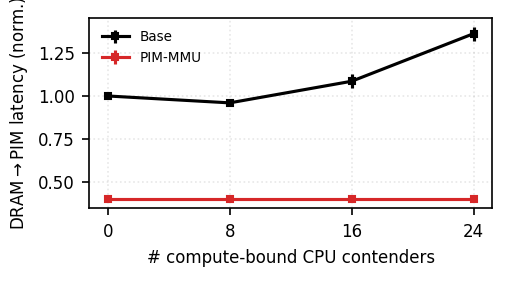
\includegraphics[width=0.78\columnwidth]{e5_contention.png}
\caption{\dtp{} latency (normalized) vs.\ number of compute-bound CPU
contenders (cf.\ paper Fig.~13a).}
\label{fig:e5}
\end{figure}

\subsection{Why the baseline loses: scheduling and timelines}
Figure~\ref{fig:e6} plots per-channel PIM-write throughput over time. The
software baseline (locality map) concentrates traffic on a few channels at a
time, because the OS schedules its transfer threads for fairness and lets some
channels run hot for whole time slices --- the coarse-grained congestion the
paper illustrates in Fig.~6 and Fig.~12. PIM-MMU spreads writes evenly across
all channels for the whole transfer. We quantify the imbalance as the mean
per-window coefficient of variation across channels; it is far higher for the
baseline than for PIM-MMU.

\begin{figure}[t]
\centering
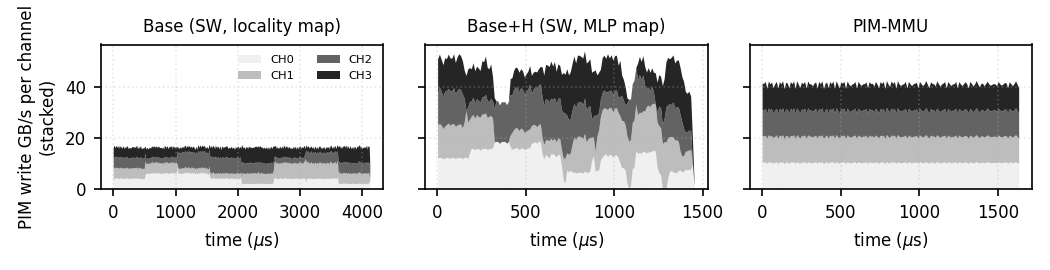
\includegraphics[width=\columnwidth]{e6_timeline.png}
\caption{Per-channel PIM-write throughput over time. The software baseline leaves
channels idle in turn; PIM-MMU keeps all channels busy (cf.\ paper Figs.~6,~12).}
\label{fig:e6}
\end{figure}

\subsection{Two places we disagree with the paper}
\label{sec:differ}
A reproduction is more useful when it is honest about where it does not line up.
Two of our results tell a slightly different story, and both have a cause we
could pin down.

The first is about which component matters most. In the paper, PIM-MS is the
headline; the scheduler is what unlocks the throughput. On our setup the DRAM
mapping does more of the work: the +H point --- software copier, but with the
MLP-centric mapping swapped in --- already reaches about $44$\,GB/s, most of the
way to full PIM-MMU. We think this is a property of our model rather than a
contradiction. The paper runs on hardware where CPU issue width and OS
scheduling put a hard ceiling on the software path, so changing only the mapping
cannot get very far. Our +H keeps an idealized software issuer and changes just
the mapping, which flatters the mapping. The paper's claim still holds in the
sense that matters: with the locality mapping, PIM-MS alone (+D+P) is poor, and
full PIM-MMU needs the scheduler to reach its peak. The two are complementary;
we only put the emphasis in a different place, and we know why.

The second is the shape of the size curve. Our PIM-MMU throughput climbs to
about $70$\,GB/s at $4$\,MB and then eases back to a $\sim$$45$\,GB/s plateau,
whereas the paper's Fig.~15(a) keeps climbing toward the large sizes. We chased
this down with per-bank row-change counters (the \texttt{-{}-debug} output) and
it is not a bug. The $4$\,MB peak is a transient: at that size all $64$ bank
units happen to be in flight together. At larger sizes the $16$\,KB data buffer
only holds about $32$ chunks, so fewer units overlap and the effective MLP
drops to a steady level --- around $58\%$ of PIM peak, and unchanged no matter
how much bigger we make the window past that point. In short, the plateau is the
honest steady-state number for a scheduler bounded by a small on-chip buffer,
and that is what we report.

\section{Our Extension: Dropping the Padding}
\subsection{Why the fixed size hurts}
Both UPMEM's API and PIM-MMU's move the \emph{same} number of bytes to every
DPU. That is fine when the work splits evenly, but a lot of interesting work does
not: sparse matrices, graphs, and histograms all hand some cores far more than
others. When that happens the programmer has only one option --- pad every DPU up
to the size of the biggest one --- and the transfer then spends real DRAM-read
and PIM-write bandwidth shuttling padding that no core will ever read. The paper
sidesteps this by evaluating only equal-sized partitions, so the cost never
appears. It seemed like the natural place to push on the design.

\subsection{What we added}
The fix has three parts, and they stack. Each lives in the DCE model, so we could
switch them on one at a time and watch what each one buys.
\begin{enumerate}
\item \textbf{Ragged descriptors.} Each descriptor carries its own byte count,
so a DPU only receives its real partition. The chunk generator stops at each
DPU's true length instead of a global padded length.
\item \textbf{Largest-remaining-first (LRF) scheduling.} Instead of Algorithm~1's
round-robin, PIM-MS picks the bank unit with the most work left (subject to a
small per-unit in-flight cap), so the heaviest units start first and stay
saturated while lighter units fill the gaps --- a longest-processing-time
schedule that minimizes the makespan tail.
\item \textbf{Size-aware placement.} A permutation chosen at transfer setup
packs eight similarly sized partitions into each bank unit (so a unit's cost,
which is the max of its 8 DPUs, is not inflated by one large outlier) and then
assigns bank units to channels by longest-processing-time, equalizing per-channel
load.
\end{enumerate}
Only the third part sends data to a different core than it otherwise would. That
is allowed because the PIM core ID is just a label the runtime assigns, and it is
cheap --- a sort of the partitions and a greedy assignment over the $64$ bank
units, done once before the transfer begins.

\subsection{Results}
We evaluate four per-DPU size distributions at a fixed 16\,KB mean over 512 DPUs:
\textbf{uniform} (sanity check), \textbf{lognormal} with $\sigma\in\{0.5,1.0\}$,
and an \textbf{R-MAT} row partition representative of SpMV/BFS (skew
max/mean~$\approx$43). We report \emph{effective} throughput (useful bytes over
time; padded bytes do not count).

Figure~\ref{fig:e8} summarizes. On uniform sizes the extension is neutral, as it
should be. On the R-MAT partition, effective \dtp{} throughput rises from
$1.54$\,GB/s for padded PIM-MMU to $7.2$\,GB/s with ragged descriptors,
$7.9$\,GB/s adding LRF, and $16.6$\,GB/s adding placement --- a $10.8\times$
gain, reaching the per-DPU bank-bandwidth bound. On the lognormal-$\sigma$1.0
case it rises from $7.0$ to $52.0$\,GB/s, and padded software (SW-pad) manages
only $0.40$\,GB/s on R-MAT, so the full extension is $41\times$ over the
software path. Figure~\ref{fig:e9} sweeps
the LRF in-flight cap: a cap of 4--6 chunks per bank unit is best; too small
starves MLP, too large reverts to a FIFO that re-creates tail imbalance.

An instructive side effect: with ragged descriptors the DRAM read traffic and the
PIM write traffic are no longer equal. Reads fetch only the useful bytes, but a
write burst still covers all eight DPUs of a bank unit, so a unit writes
$\max(\text{8 DPUs})\times 8$ bursts regardless of how little some of those DPUs
need. On the lognormal-$\sigma$1.0 input the write side therefore moves
$2.97\times$ the read side. This is exactly why placement matters: by grouping
similarly sized partitions into a unit it shrinks that write-side padding (the
ratio falls from $1.85$ to $1.03$ on lognormal-$\sigma$0.5), which is visible as
the large jump from \texttt{+Ragged} to \texttt{+Ragged+Place} in
Fig.~\ref{fig:e8}. A naive ``bytes read $=$ bytes written'' check will flag every
skewed ragged run; the correct invariant is that reads equal the useful payload
and writes equal the useful payload times the placement's padding ratio.

\begin{figure}[t]
\centering
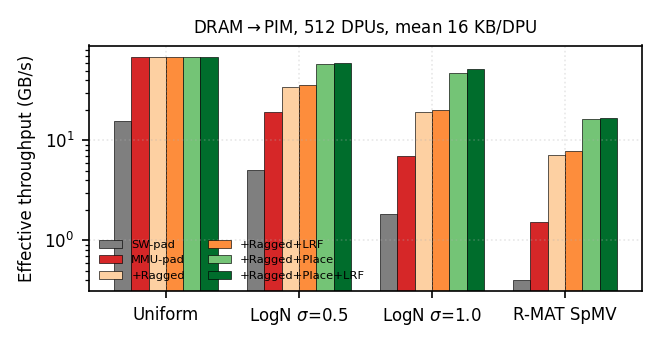
\includegraphics[width=\columnwidth]{e8_extension.png}
\caption{Effective throughput (useful bytes/s, log scale) for four per-DPU size
distributions. The extension is neutral on uniform sizes and large on skewed
ones; placement is the dominant lever for heavy skew.}
\label{fig:e8}
\end{figure}

\begin{figure}[t]
\centering
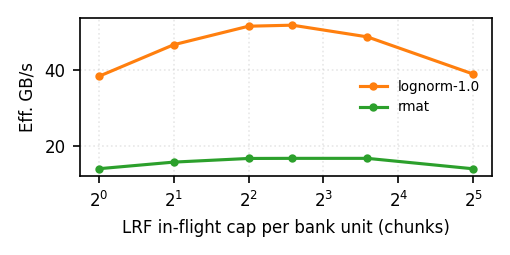
\includegraphics[width=0.78\columnwidth]{e9_lrfcap.png}
\caption{Effect of the LRF in-flight cap per bank unit on effective throughput.}
\label{fig:e9}
\end{figure}

\section{Limitations and Threats to Validity}
\label{sec:threats}
\begin{itemize}
\item \textbf{No real hardware.} Every number here is from simulation. We did not
run UPMEM, so we cannot validate absolute latencies against silicon; we validate
\emph{trends} and, where possible, cross-check against the paper's reported
numbers (e.g.\ our large-transfer baseline's $8.3$\,GB/s is close to the paper's $8.9$\,GB/s).
\item \textbf{Channel count and DIMM model.} We use 4+4 channels where the
paper's server has 3+3, and we approximate UPMEM's 8-banks-per-chip organization
with a DDR4 x16 geometry. These choices shift absolute bandwidths and explain
why our locality-vs-MLP ratio is 18\% vs.\ the paper's 30\% and why our memcpy
speedups differ slightly from $4.9\times$.
\item \textbf{Idealized software model.} Our Base models AVX issue, LFB limits
and OS time-slicing but not cache pollution, TLB effects, or real AVX-512
frequency throttling. This likely makes Base optimistic, which in turn makes our
+H point over-credit the DRAM mapping (Section~\ref{sec:differ}).
\item \textbf{Transpose and preprocessing} are modeled as a fixed latency, not a
gate-level unit; we did not estimate its area or power (left out by assignment).
\item \textbf{Left out} (restating): PIM kernel execution, driver/runtime,
power/area, and end-to-end PrIM times.
\end{itemize}

\section{Related Work}
PIM-MMU builds on a long line of PIM characterization and memory-management work;
we refer the reader to the original paper~\cite{pimmmu} for the full
treatment. Our DCE resembles DMA engines (Intel I/OAT/DSA) but, as the paper and
our +D ablation show, a plain DMA engine underperforms the baseline on this
problem. Our ragged-transfer extension is related to load-balancing in sparse
PIM kernels (SparseP) and to longest-processing-time scheduling, applied here to
the data-transfer layer rather than the compute layer.

\section{Conclusion}
Working only from the paper, with none of its code, we rebuilt the DRAM$\,
\leftrightarrow\,$PIM transfer path in Ramulator and got the same story back out
of it: full PIM-MMU is several times faster than the software copier, a bare copy
engine is \emph{slower} than the software it replaces, HetMap does nothing until
PIM-MS is scheduling behind it, and the software baseline both wilts under CPU
contention and uses the memory channels unevenly. Two of our numbers come out
differently from the paper's, and rather than paper over that we tracked each to
its cause --- the idealization in our software model, and the small on-chip
buffer that caps steady-state parallelism. Finally we took the design somewhere
it does not currently go. By dropping the per-DPU padding and adding
largest-remaining scheduling and size-aware placement, we recovered up to
$10.8\times$ effective throughput on badly skewed partitions, and lost nothing on
even ones. For the many PIM workloads that are irregular by nature, that gap
looks worth closing.

\section*{Contributions of Team Members}
\begin{itemize}
\item \textbf{Sunil:} Ramulator integration, DDR4 configuration, address-mapping
functions (locality and MLP-centric with XOR hashing), and the two-line
controller patch.
\item \textbf{Subham:} Software baseline model (cores, LFBs, OS scheduler) and
the DCE/PIM-MS implementation of Algorithm~1; baseline experiments E1--E2.
\item \textbf{Shrey Chandra:} HetMap, microbenchmarks (memcpy, stream, contention),
timelines, and the paper-comparison experiments E3--E7.
\item \textbf{Jagratti:} Ragged-transfer extension (ragged descriptors, LRF,
placement), its experiments E8--E9, plotting, and the report write-up.
\end{itemize}
\emph{All members jointly debugged the 64\,MB plateau and reviewed the final report.}

\balance
\begin{thebibliography}{00}
\bibitem{pimmmu} D. Lee, B. Hyun, T. Kim, and M. Rhu, ``PIM-MMU: A Memory
Management Unit for Accelerating Data Transfers in Commercial PIM Systems,''
\emph{MICRO}, 2024.
\bibitem{upmem} F. Devaux, ``The True Processing In Memory Accelerator,''
\emph{Hot Chips}, 2019.
\bibitem{prim} J. G\'omez-Luna \emph{et al.}, ``Benchmarking a New Paradigm: An
Experimental Analysis of a Real Processing-in-Memory Architecture,'' 2021.
\bibitem{ramulator} Y. Kim, W. Yang, and O. Mutlu, ``Ramulator: A Fast and
Extensible DRAM Simulator,'' \emph{IEEE CAL}, 2015.
\bibitem{xorhash} Z. Zhang, Z. Zhu, and X. Zhang, ``A Permutation-Based Page
Interleaving Scheme to Reduce Row-Buffer Conflicts and Exploit Data Locality,''
\emph{MICRO}, 2000.
\end{thebibliography}

\end{document}
